% !TeX root = ../main.tex
% ============================================================
% LÁMINA 8 — ETAPA 1: CAPTURA (fondo claro)
% ============================================================
\begin{frame}[plain]
  \begin{tikzpicture}[remember picture, overlay]

    \fill[paperBg] (current page.south west) rectangle (current page.north east);

    \node[anchor=north west, align=left]
      at ([xshift=1.4cm, yshift=-0.55cm]current page.north west)
      {\kicker[accentBlue]{07 \,$\cdot$\, Caso clínico \,$\cdot$\, Etapa 1}};

    \node[anchor=north west, align=left, text width=13.2cm]
      at ([xshift=1.4cm, yshift=-1.05cm]current page.north west)
      {\large\bfseries\sffamily\color{inkText}La app transmite el audio en tiempo real por \textit{WebSocket} seguro};

    % ------------------------------------------------------
    % Breadcrumb de 6 etapas (Captura resaltada)
    % ------------------------------------------------------
    \def\bcW{2.05cm}
    \def\bcH{0.5cm}
    \def\bcGap{0.16cm}
    \def\bcStep{2.21cm}
    \def\bcY{-1.85cm}

    \node[anchor=north west, fill=inkDark, rounded corners=8pt,
          minimum width=\bcW, minimum height=\bcH, align=center, inner sep=0pt]
      at ([xshift=1.4cm+0*\bcStep, yshift=\bcY]current page.north west)
      {\fontsize{6.5}{6.5}\selectfont\bfseries\sffamily\color{accentTeal}1\,\textperiodcentered\,Captura};

    \node[anchor=north west, fill=cardWhite, draw=lineGrey, line width=0.6pt, rounded corners=8pt,
          minimum width=\bcW, minimum height=\bcH, align=center, inner sep=0pt]
      at ([xshift=1.4cm+1*\bcStep, yshift=\bcY]current page.north west)
      {\fontsize{6.5}{6.5}\selectfont\bfseries\sffamily\color{mutedText}2\,\textperiodcentered\,ASR};

    \node[anchor=north west, fill=cardWhite, draw=lineGrey, line width=0.6pt, rounded corners=8pt,
          minimum width=\bcW, minimum height=\bcH, align=center, inner sep=0pt]
      at ([xshift=1.4cm+2*\bcStep, yshift=\bcY]current page.north west)
      {\fontsize{6.5}{6.5}\selectfont\bfseries\sffamily\color{mutedText}3\,\textperiodcentered\,NER};

    \node[anchor=north west, fill=cardWhite, draw=lineGrey, line width=0.6pt, rounded corners=8pt,
          minimum width=\bcW, minimum height=\bcH, align=center, inner sep=0pt]
      at ([xshift=1.4cm+3*\bcStep, yshift=\bcY]current page.north west)
      {\fontsize{6.5}{6.5}\selectfont\bfseries\sffamily\color{mutedText}4\,\textperiodcentered\,Normaliz.};

    \node[anchor=north west, fill=cardWhite, draw=lineGrey, line width=0.6pt, rounded corners=8pt,
          minimum width=\bcW, minimum height=\bcH, align=center, inner sep=0pt]
      at ([xshift=1.4cm+4*\bcStep, yshift=\bcY]current page.north west)
      {\fontsize{6.5}{6.5}\selectfont\bfseries\sffamily\color{mutedText}5\,\textperiodcentered\,Generación};

    \node[anchor=north west, fill=cardWhite, draw=lineGrey, line width=0.6pt, rounded corners=8pt,
          minimum width=\bcW, minimum height=\bcH, align=center, inner sep=0pt]
      at ([xshift=1.4cm+5*\bcStep, yshift=\bcY]current page.north west)
      {\fontsize{6.5}{6.5}\selectfont\bfseries\sffamily\color{mutedText}6\,\textperiodcentered\,Validación};

    % ------------------------------------------------------
    % Capturas reales de la app móvil
    % ------------------------------------------------------
    \coordinate (shot1TL) at ([xshift=1.4cm, yshift=-2.65cm]current page.north west);
    \begin{scope}
      \clip [rounded corners=4pt] (shot1TL) rectangle ($(shot1TL)+(3.75cm,-3.9cm)$);
      \node[anchor=north west, inner sep=0pt] at (shot1TL)
        {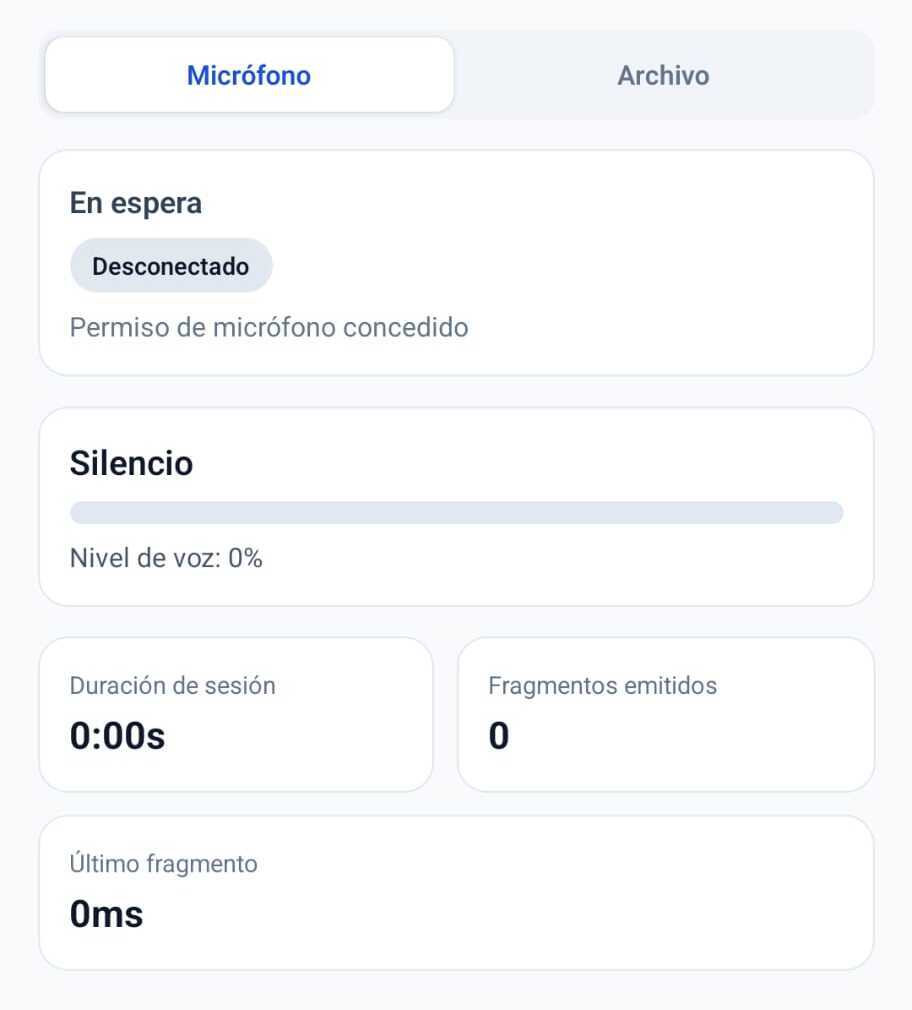
\includegraphics[width=3.75cm]{imagenes/app_idle_crop.jpeg}};
    \end{scope}
    \draw[lineGrey, line width=0.8pt, rounded corners=4pt]
      (shot1TL) rectangle ($(shot1TL)+(3.75cm,-3.9cm)$);
    \node[anchor=north west, align=left]
      at ([yshift=-4.1cm]shot1TL)
      {\fontsize{7}{7}\selectfont\bfseries\sffamily\color{mutedText}En espera};

    \coordinate (shot2TL) at ([xshift=3.95cm]shot1TL);
    \begin{scope}
      \clip [rounded corners=4pt] (shot2TL) rectangle ($(shot2TL)+(3.75cm,-3.9cm)$);
      \node[anchor=north west, inner sep=0pt] at (shot2TL)
        {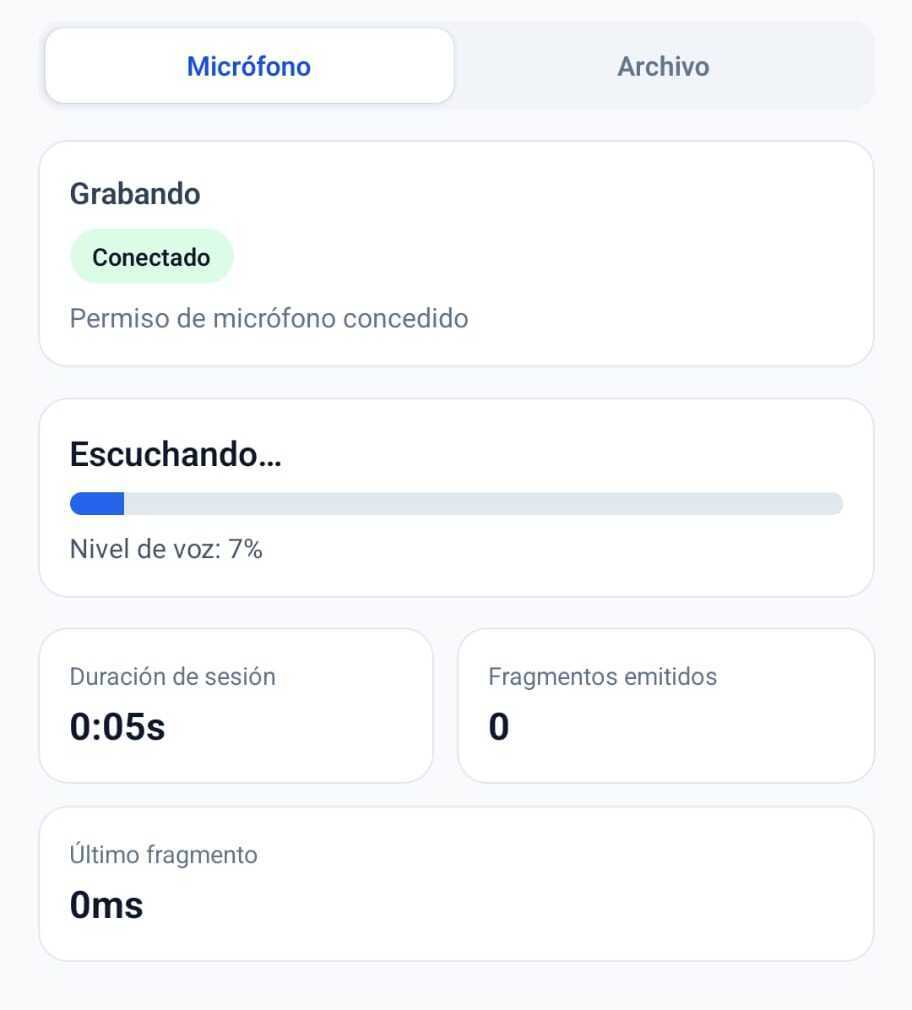
\includegraphics[width=3.75cm]{imagenes/app_sending_crop.jpeg}};
    \end{scope}
    \draw[lineGrey, line width=0.8pt, rounded corners=4pt]
      (shot2TL) rectangle ($(shot2TL)+(3.75cm,-3.9cm)$);
    \node[anchor=north west, align=left]
      at ([yshift=-4.1cm]shot2TL)
      {\fontsize{7}{7}\selectfont\bfseries\sffamily\color{mutedText}Grabando};

    % ------------------------------------------------------
    % 3 bullets a la derecha
    % ------------------------------------------------------
    \def\bulX{9.45cm}
    \def\bulTextW{5.1cm}

    % Cada párrafo se ancla debajo del anterior (altura variable), y el
    % círculo se posiciona relativo a su propio texto.
    \node[anchor=north west] (bt1)
      at ([xshift=\bulX, yshift=-2.68cm]current page.north west)
      {\parbox[t]{\bulTextW}{\raggedright\small\bfseries\sffamily\color{inkText}Conexión \textit{WSS} de extremo a extremo\\[1pt]
       \fontsize{8}{9.5}\selectfont\normalfont\color{mutedText}%
       Cifrada desde el primer fragmento de audio}};

    \node[anchor=north west] (bt2)
      at ([yshift=-0.22cm]bt1.south west)
      {\parbox[t]{\bulTextW}{\raggedright\small\bfseries\sffamily\color{inkText}Audio \textit{PCM} en bloques de $\sim$250\,ms\\[1pt]
       \fontsize{8}{9.5}\selectfont\normalfont\color{mutedText}%
       Procesamiento incremental sin esperar al final}};

    \node[anchor=north west] (bt3)
      at ([yshift=-0.22cm]bt2.south west)
      {\parbox[t]{\bulTextW}{\raggedright\small\bfseries\sffamily\color{inkText}Estado visible en tiempo real\\[1pt]
       \fontsize{8}{9.5}\selectfont\normalfont\color{mutedText}%
       Conexión, nivel de voz y fragmentos emitidos}};

    % ------------------------------------------------------
    % Caja de cierre
    % ------------------------------------------------------
    % \coordinate (closeAnchor) at (current page.north west |- bt3.south west);
    % \node[anchor=north west, fill=inkDark, rounded corners=6pt,
    %       minimum width=13.2cm, minimum height=1.4cm, align=left, inner sep=0pt]
    %   (closebox) at ([xshift=1.4cm, yshift=-0.3cm]closeAnchor) {};
    % \node[anchor=west, align=left, text width=12.4cm]
    %   at ([xshift=0.4cm]closebox.west)
    %   {\small\sffamily\color{white}%
    %    Para el Caso 1, la app capturó y transmitió el dictado completo sin pérdida de
    %    fragmentos: la sesión llegó íntegra a la etapa de \textit{ASR}.};

  \end{tikzpicture}
  \end{frame}
